% begin module limits-ex7
\begin{frame}
By comparing the definitions, we can see that
\[
\lim_{x\rightarrow a} f(x) = L \ \text{ if and only if } \lim_{x\rightarrow a^-}f(x) = L \ \text{ and } \lim_{x\rightarrow a^+}f(x) = L .
\]
\begin{example} %[Example 7, p. 100]
\begin{columns}[c]
\column{.55\textwidth}
The graph of a function $g$ is shown to the right.  Use it to state the values (if they exist) of the following:
\begin{align*}
\alert<handout:0| 2-3>{\lim_{x\rightarrow 1^-}g(x)} & \alert<handout:0 |2-3>{=} \alert<handout:0 |3>{\uncover<3->{3}} &%
\alert<handout:0| 8-9>{\lim_{x\rightarrow 3^-}g(x)} & \alert<handout:0 |8-9>{=} \alert<handout:0 |9>{\uncover<9->{1}} \\%
\alert<handout:0| 4-5>{\lim_{x\rightarrow 1^+}g(x)} & \alert<handout:0 |4-5>{=} \alert<handout:0 |5>{\uncover<5->{3}} &%
\alert<handout:0| 10-11>{\lim_{x\rightarrow 3^+}g(x)} & \alert<handout:0 |10-11>{=} \alert<handout:0 |11>{\uncover<11->{2}} \\%
\alert<handout:0| 6-7>{\lim_{x\rightarrow 1}g(x)} & \alert<handout:0 |6-7>{=} \alert<handout:0 |7>{\uncover<7->{3}} &%
\alert<handout:0| 12-13>{\lim_{x\rightarrow 3}g(x)} & \alert<handout:0 |12-13>{=} %
 \uncover<13->{\alert<handout:0| 13>{\text{DNE}}} %
\end{align*}
\column{.45\textwidth}
\psset{xunit=0.9cm, yunit=0.9cm}
\begin{pspicture}(-0.5, -0.5)(5.3,5.1) 
\psframe*[linecolor=white](-0.5,-0.5)(5.3,5.1)
\tiny 
\psaxes{<->}(0,0)(-0.5,-0.5)(5.2,5)
\psLabels{5.2}{5}
%Function formula: 37/10+9/20 (x)+7/20 ((x)^{3})-3/2 ((x)^{2}) 
\psplot[linecolor=red, plotpoints=1000]{-0.5}{3}{x 2 exp -1.5 mul x 3 exp 0.35 mul x 0.45 mul 3.7 add add add }
%Function formula: 3/2+1/2 ((-4+x)^{2}) 
\psplot[linecolor=red, plotpoints=1000]{3}{5}{x -4 add 2 exp 0.5 mul 1.5 add }
\rput[lb](1.6,2.3){$y=g(x)$}
\psFullDot{1}{4}
\psHollowDot{1}{3}
\psHollowDot{3}{1}
\psHollowDot{3}{2}
\end{pspicture} 
% 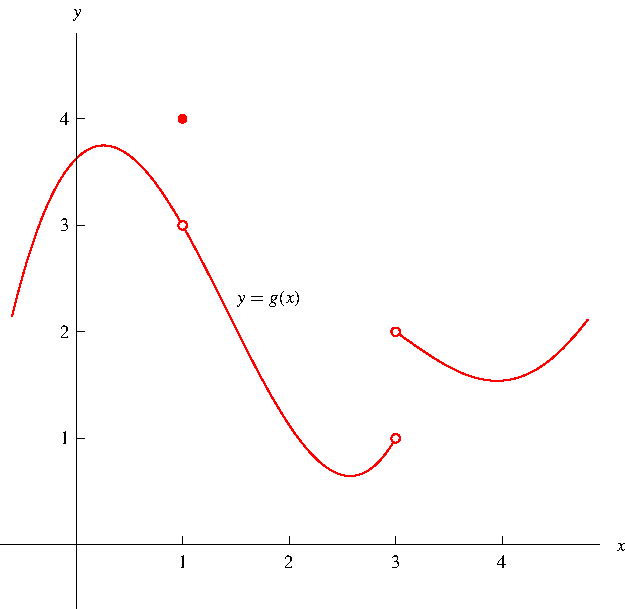
\includegraphics[height=5cm]{limits/pictures/02-02-ex7.pdf}%
\end{columns}
\end{example}
\end{frame}
% end module limits-ex7
